% filepath: pre_test_v6_shared_gamma_documentation.tex
\documentclass[a4paper,12pt,dvipdfmx]{jlreq}
\usepackage{amsmath,amssymb,amsthm}
\usepackage{bm}
\usepackage{physics}
\usepackage{tikz}
\usetikzlibrary{shapes.geometric, arrows, positioning, fit, backgrounds}
\usepackage{algorithm2e}
\usepackage{booktabs}
\usepackage{graphicx}
\usepackage{hyperref}
\usepackage{xcolor}
\usepackage{tcolorbox}
\usepackage{listings}
\usepackage{siunitx}
\usepackage{multirow}

% カラーボックス設定
\newtcolorbox{keypoint}{colback=blue!5!white,colframe=blue!75!black,title=Key Point}
\newtcolorbox{warning}{colback=red!5!white,colframe=red!75!black,title=注意}
\newtcolorbox{definition}{colback=green!5!white,colframe=green!50!black,title=定義}

\lstset{
    basicstyle=\footnotesize\ttfamily,
    keywordstyle=\color{blue},
    commentstyle=\color{gray},
    breaklines=true,
    frame=single
}

\title{\vspace{-2cm}
\textbf{pre\_test\_v6\_shared\_gamma.py 理解ドキュメント}\\
\large 共有γモデルによるテラヘルツ透過スペクトル解析
}
\author{物理工学専攻 修士論文解析用教材}
\date{2026年1月版}

\begin{document}
\maketitle

\tableofcontents
\clearpage

%%%%%%%%%%%%%%%%%%%%%%%%%%%%%%%%%%%%%%%%%%%%%%%%%%%%%%%%%%%%%%%%%
\section{はじめに:このプログラムの目的}
%%%%%%%%%%%%%%%%%%%%%%%%%%%%%%%%%%%%%%%%%%%%%%%%%%%%%%%%%%%%%%%%%

\begin{keypoint}
このプログラムは、Gd$_3$Ga$_5$O$_{12}$(GGG)ガーネット結晶のテラヘルツ透過スペクトルを、
\textbf{共有γ(ガンマ)モデル}を用いて全データセットを同時にフィッティングするためのものです。
\end{keypoint}

\subsection{背景:何を解決しようとしているか}

テラヘルツ分光実験では、異なる温度$T$や磁場$B$の条件で透過スペクトルを測定します。
各スペクトルを個別にフィッティングすると、パラメータ数が膨大になり:

\begin{itemize}
    \item \textbf{v4モデル}: 75個のパラメータ(5 global + 70 local gamma)
    \item 条件数(Condition Number): $\kappa \approx 10^{16}$(数値的に非常に不安定)
    \item パラメータ間の相関が高く、物理的解釈が困難
\end{itemize}

\subsection{本プログラムの革新点}

\begin{definition}
\textbf{共有γモデル(v6)}は、全データセットで7個の緩和率$\gamma_k$($k=0,1,\ldots,6$)を共有することで、
パラメータ数を大幅に削減します:
\[
\boxed{\text{パラメータ数}: 75個 \to 12個 \quad (\text{84\%削減})}
\]
\end{definition}

物理的根拠:緩和率$\gamma_k$は材料固有の特性であり、温度・磁場によらないと仮定。

%%%%%%%%%%%%%%%%%%%%%%%%%%%%%%%%%%%%%%%%%%%%%%%%%%%%%%%%%%%%%%%%%
\section{物理モデルの概要}
%%%%%%%%%%%%%%%%%%%%%%%%%%%%%%%%%%%%%%%%%%%%%%%%%%%%%%%%%%%%%%%%%

\subsection{対象系:Gd$^{3+}$イオンの電子スピン}

Gd$^{3+}$イオンは電子配置$[\text{Xe}]4f^7$を持ち、スピン量子数$S=7/2$です。
これにより、$2S+1=8$個のスピン状態($|m\rangle$, $m=7/2, 5/2, \ldots, -7/2$)が存在します。

\begin{figure}[h]
\centering
\begin{tikzpicture}[scale=0.8]
    % エネルギー準位図
    \foreach \i/\label/\energy in {0/$|0\rangle$/0, 1/$|1\rangle$/1.2, 2/$|2\rangle$/2.5, 3/$|3\rangle$/3.9, 4/$|4\rangle$/5.4, 5/$|5\rangle$/7.0, 6/$|6\rangle$/8.7, 7/$|7\rangle$/10.5} {
        \draw[thick] (0,\energy) -- (3,\energy);
        \node[left] at (0,\energy) {\label};
        \node[right] at (3,\energy) {$E_\i$};
    }
    % 遷移矢印(例)
    \draw[->,red,thick] (1.5,0) -- (1.5,1.2) node[midway,right] {$\gamma_0$};
    \draw[->,blue,thick] (2,1.2) -- (2,2.5) node[midway,right] {$\gamma_1$};
    
    % 軸ラベル
    \draw[->] (-0.5,0) -- (-0.5,11) node[above] {Energy};
    
    % 説明
    \node[align=center] at (6,5) {\textbf{8準位系}\\$S = 7/2$\\\\各準位に固有の\\緩和率$\gamma_k$};
\end{tikzpicture}
\caption{Gd$^{3+}$イオンの8準位エネルギー図。各準位$|k\rangle$には固有の緩和率$\gamma_k$が割り当てられる。}
\label{fig:energy_levels}
\end{figure}

%%%%%%%%%%%%%%%%%%%%%%%%%%%%%%%%%%%%%%%%%%%%%%%%%%%%%%%%%%%%%%%%%
\section{ハミルトニアンの構築}
%%%%%%%%%%%%%%%%%%%%%%%%%%%%%%%%%%%%%%%%%%%%%%%%%%%%%%%%%%%%%%%%%

\subsection{全ハミルトニアン}

系のハミルトニアン$\hat{H}$は、結晶場項とゼーマン項の和で与えられます:

\begin{equation}
\boxed{
\hat{H} = \hat{H}_{\text{CF}} + \hat{H}_{\text{Zee}}
}
\label{eq:total_hamiltonian}
\end{equation}

\subsection{結晶場ハミルトニアン $\hat{H}_{\text{CF}}$}

GGGの立方対称性を反映し、Stevens演算子を用いて表されます:

\begin{equation}
\hat{H}_{\text{CF}} = B_4 \left( \hat{O}_4^0 + 5\hat{O}_4^4 \right) + B_6 \left( \hat{O}_6^0 - 21\hat{O}_6^4 \right)
\label{eq:cf_hamiltonian}
\end{equation}

ここで:
\begin{itemize}
    \item $B_4, B_6$: 結晶場パラメータ(単位:K)
    \item $\hat{O}_l^m$: Stevens演算子(無次元)
\end{itemize}

\begin{keypoint}
Stevens演算子$\hat{O}_l^m$は、$8 \times 8$行列として表現されます。コード中では:
\begin{lstlisting}[language=Python]
# O40演算子(対角成分のみ)
O40 = np.diag([7, -13, -3, 9, 9, -3, -13, 7]) / 60

# O44演算子(非対角成分)
X_O44[3, 7] = X_O44[4, 0] = np.sqrt(35) / 12
X_O44[2, 6] = X_O44[5, 1] = 5 * np.sqrt(3) / 12
O44 = (X_O44 + X_O44.T)
\end{lstlisting}
\end{keypoint}

\subsection{ゼーマン項 $\hat{H}_{\text{Zee}}$}

外部磁場$B$下での磁気エネルギー:

\begin{equation}
\hat{H}_{\text{Zee}} = g \mu_{\text{B}} B \hat{S}_z
\label{eq:zeeman}
\end{equation}

ここで:
\begin{itemize}
    \item $g$: ランデg因子($\approx 2.0$)
    \item $\mu_{\text{B}} = 9.274 \times 10^{-24}$ J/T: ボーア磁子
    \item $\hat{S}_z$: スピンz成分演算子
\end{itemize}

\begin{warning}
単位系に注意!コード中では温度単位[K]に統一されています:
\[
\hat{H}_{\text{Zee}} [\text{K}] = \frac{g \mu_{\text{B}} B \hat{S}_z}{k_{\text{B}}}
\]
ここで$k_{\text{B}} = 1.381 \times 10^{-23}$ J/Kはボルツマン定数。
\end{warning}

\subsection{固有値問題}

ハミルトニアン行列を対角化して固有値(エネルギー)と固有ベクトル(状態)を求めます:

\begin{equation}
\hat{H} |n\rangle = E_n |n\rangle \quad (n = 0, 1, \ldots, 7)
\end{equation}

コード実装:
\begin{lstlisting}[language=Python]
E_vals, U = np.linalg.eigh(H)  # Hermite行列の対角化
\end{lstlisting}

%%%%%%%%%%%%%%%%%%%%%%%%%%%%%%%%%%%%%%%%%%%%%%%%%%%%%%%%%%%%%%%%%
\section{磁気感受率の計算}
%%%%%%%%%%%%%%%%%%%%%%%%%%%%%%%%%%%%%%%%%%%%%%%%%%%%%%%%%%%%%%%%%

\subsection{線形応答理論}

周波数$\omega$の交流磁場に対する磁気感受率$\chi(\omega)$は、久保公式に基づいて計算されます。
全$8 \times 7 = 56$個の遷移ペア$(n \leftrightarrow n')$の寄与を合計します:

\begin{equation}
\boxed{
\chi(\omega) = \sum_{n < n'} \frac{(p_n - p_{n'}) \cdot |\langle n | \hat{S}_\perp | n' \rangle|^2}{\omega_{nn'} - \omega - i\gamma_{k}}
}
\label{eq:susceptibility}
\end{equation}

ここで:
\begin{itemize}
    \item $p_n$: 準位$|n\rangle$のボルツマン占有確率
    \item $\omega_{nn'} = (E_{n'} - E_n)/\hbar$: 遷移周波数
    \item $\hat{S}_\perp = (\hat{S}_x + \hat{S}_y)/2$: 面内スピン成分
    \item $\gamma_k$: 初期状態$|k\rangle$の緩和率(\textbf{7-gamma方式})
\end{itemize}

\subsection{ボルツマン分布}

温度$T$における準位占有確率は:

\begin{equation}
p_n = \frac{e^{-E_n / k_{\text{B}} T}}{Z}, \quad Z = \sum_{n=0}^{7} e^{-E_n / k_{\text{B}} T}
\label{eq:boltzmann}
\end{equation}

\begin{figure}[h]
\centering
\begin{tikzpicture}[scale=0.9]
    % 低温
    \begin{scope}
        \draw[->] (0,0) -- (0,4) node[above] {$p_n$};
        \draw[->] (0,0) -- (4.5,0) node[right] {$n$};
        \foreach \x in {0,1,2,3,4,5,6,7} {
            \draw (\x*0.5+0.25,0.1) -- (\x*0.5+0.25,-0.1) node[below] {\small\x};
        }
        % 低温での分布
        \fill[blue!60] (0.25,0) rectangle (0.75,3.5);
        \fill[blue!40] (0.75,0) rectangle (1.25,0.4);
        \fill[blue!20] (1.25,0) rectangle (1.75,0.05);
        \node[below] at (2,-0.8) {\textbf{低温 $T \ll E_1/k_{\text{B}}$}};
        \node at (2.2,2.5) {$p_0 \approx 1$};
    \end{scope}
    
    % 高温
    \begin{scope}[xshift=7cm]
        \draw[->] (0,0) -- (0,4) node[above] {$p_n$};
        \draw[->] (0,0) -- (4.5,0) node[right] {$n$};
        \foreach \x in {0,1,2,3,4,5,6,7} {
            \draw (\x*0.5+0.25,0.1) -- (\x*0.5+0.25,-0.1) node[below] {\small\x};
        }
        % 高温での分布
        \foreach \x in {0,1,2,3,4,5,6,7} {
            \fill[red!50] (\x*0.5+0.1,0) rectangle (\x*0.5+0.4,1.0);
        }
        \node[below] at (2,-0.8) {\textbf{高温 $T \gg E_7/k_{\text{B}}$}};
        \node at (2.2,2.5) {$p_n \approx 1/8$};
    \end{scope}
\end{tikzpicture}
\caption{ボルツマン分布の温度依存性。低温では基底状態に集中し、高温では均等に分布する。}
\label{fig:boltzmann}
\end{figure}

\subsection{7-gamma初期状態ベース方式}

\begin{definition}
本モデルの核心である\textbf{7-gamma方式}では、56個の遷移を7個のパラメータで記述します:

遷移$|n\rangle \leftrightarrow |n'\rangle$に対して、エネルギーが低い方の準位のγを使用:
\[
\gamma_{\text{transition}} = \gamma_{\min(n,n')}
\]
\end{definition}

この物理的意味は、緩和過程が主に初期状態(低エネルギー側)の特性で決まるという仮定です。

\begin{figure}[h]
\centering
\begin{tikzpicture}[scale=0.8]
    % 遷移とγの対応を示す図
    \node[draw, rectangle, minimum width=2cm, minimum height=0.8cm] (g0) at (0,0) {$\gamma_0$};
    \node[draw, rectangle, minimum width=2cm, minimum height=0.8cm] (g1) at (3,0) {$\gamma_1$};
    \node[draw, rectangle, minimum width=2cm, minimum height=0.8cm] (g2) at (6,0) {$\gamma_2$};
    \node at (9,0) {$\cdots$};
    \node[draw, rectangle, minimum width=2cm, minimum height=0.8cm] (g6) at (12,0) {$\gamma_6$};
    
    % 遷移数
    \node[below=0.3cm] at (g0) {7遷移};
    \node[below=0.3cm] at (g1) {6遷移};
    \node[below=0.3cm] at (g2) {5遷移};
    \node[below=0.3cm] at (g6) {1遷移};
    
    % 矢印で準位からの遷移を示す
    \node[above=0.8cm] at (g0) {$|0\rangle \to |1,2,...,7\rangle$};
    \node[above=0.8cm] at (g1) {$|1\rangle \to |2,3,...,7\rangle$};
    \node[above=0.8cm] at (g2) {$|2\rangle \to |3,4,...,7\rangle$};
    \node[above=0.8cm] at (g6) {$|6\rangle \to |7\rangle$};
\end{tikzpicture}
\caption{7-gamma方式:各$\gamma_k$が担当する遷移数。$\gamma_0$は7個、$\gamma_6$は1個の遷移を制御。}
\label{fig:7gamma}
\end{figure}

%%%%%%%%%%%%%%%%%%%%%%%%%%%%%%%%%%%%%%%%%%%%%%%%%%%%%%%%%%%%%%%%%
\section{比透磁率と透過率の計算}
%%%%%%%%%%%%%%%%%%%%%%%%%%%%%%%%%%%%%%%%%%%%%%%%%%%%%%%%%%%%%%%%%

\subsection{比透磁率 $\mu_r$}

感受率から比透磁率への変換には、2つのモデル形式があります:

\subsubsection{H形式(線形モデル)}

\begin{equation}
\boxed{\mu_r^{(H)} = 1 + \chi}
\label{eq:H_form}
\end{equation}

物理的意味:磁化$\bm{M}$が外部磁場$\bm{H}$に比例する場合。

\subsubsection{B形式(非線形モデル)}

\begin{equation}
\boxed{\mu_r^{(B)} = \frac{1}{1 - \chi}}
\label{eq:B_form}
\end{equation}

物理的意味:磁化$\bm{M}$が磁束密度$\bm{B}$に比例する場合。

\begin{warning}
B形式では$\chi \to 1$で発散!これを防ぐため\textbf{Smart Damping}を適用:
\begin{equation}
\mu_r^{(B)} = \frac{1}{1 - \chi + i\delta} \quad \text{when } |1 - \chi| < \epsilon
\end{equation}
コード中では$\epsilon = 10^{-3}$, $\delta = 5 \times 10^{-3}$。
\end{warning}

\subsection{透過率計算(Fabry-Perot)}

試料を透過する電磁波は多重反射により干渉効果を示します。透過率は:

\begin{equation}
T(\omega) = \left| \frac{4Z}{(1+Z)^2 e^{-i\delta} - (1-Z)^2 e^{i\delta}} \right|^2
\label{eq:transmission}
\end{equation}

ここで:
\begin{align}
Z &= \sqrt{\frac{\mu_r}{\varepsilon_{\text{bg}}}} \quad \text{(複素インピーダンス比)} \\
\delta &= \frac{2\pi n_{\text{eff}} d}{\lambda_0} = \frac{\omega d \sqrt{\varepsilon_{\text{bg}} \mu_r}}{c} \quad \text{(位相遅れ)}
\end{align}

\begin{itemize}
    \item $d = 157.8$ $\mu$m: 試料厚さ
    \item $\varepsilon_{\text{bg}} \approx 14.5$: 背景誘電率
    \item $c = 3 \times 10^8$ m/s: 光速
\end{itemize}

%%%%%%%%%%%%%%%%%%%%%%%%%%%%%%%%%%%%%%%%%%%%%%%%%%%%%%%%%%%%%%%%%
\section{パラメータと最適化}
%%%%%%%%%%%%%%%%%%%%%%%%%%%%%%%%%%%%%%%%%%%%%%%%%%%%%%%%%%%%%%%%%

\subsection{全パラメータ一覧}

\begin{table}[h]
\centering
\caption{共有γモデル(v6)の全パラメータ}
\begin{tabular}{lcccc}
\toprule
\textbf{カテゴリ} & \textbf{パラメータ} & \textbf{初期値} & \textbf{範囲} & \textbf{物理的意味} \\
\midrule
\multirow{5}{*}{Global (5個)} 
 & $g$ & 1.95 & [1.80, 2.15] & ランデg因子 \\
 & $a$ & 22.0 & [10.0, 35.0] & スケーリング係数 \\
 & $B_4$ & 0.0038 K & [0.001, 0.008] & 結晶場パラメータ \\
 & $B_6$ & $-0.0001$ K & [$-0.0003$, 0] & 結晶場パラメータ \\
 & $\varepsilon_{\text{bg}}$ & 14.5 & [13.0, 16.0] & 背景誘電率 \\
\midrule
\multirow{7}{*}{Shared $\gamma$ (7個)} 
 & $\gamma_0$ & 0.10 THz & [0.005, 0.4] & 基底状態の緩和率 \\
 & $\gamma_1$ & 0.15 THz & [0.005, 0.4] & 第1励起状態の緩和率 \\
 & $\gamma_2$ & 0.12 THz & [0.005, 0.4] & 第2励起状態の緩和率 \\
 & $\gamma_3$ & 0.11 THz & [0.005, 0.4] & 第3励起状態の緩和率 \\
 & $\gamma_4$ & 0.14 THz & [0.005, 0.4] & 第4励起状態の緩和率 \\
 & $\gamma_5$ & 0.13 THz & [0.005, 0.4] & 第5励起状態の緩和率 \\
 & $\gamma_6$ & 0.16 THz & [0.005, 0.4] & 第6励起状態の緩和率 \\
\bottomrule
\end{tabular}
\label{tab:parameters}
\end{table}

\subsection{パラメータスケーリング}

最適化の数値安定性を向上させるため、各パラメータにスケーリング係数を適用:

\begin{equation}
\theta_{\text{scaled}} = \theta_{\text{physical}} \times S_\theta
\end{equation}

\begin{table}[h]
\centering
\caption{スケーリング係数}
\begin{tabular}{lcc}
\toprule
\textbf{パラメータ} & \textbf{スケーリング係数 $S$} & \textbf{スケール後の範囲} \\
\midrule
$g$ & 2.0 & [3.6, 4.3] \\
$a$ & 20.0 & [200, 700] \\
$B_4$ & 200.0 & [0.2, 1.6] \\
$B_6$ & 10000.0 & [$-3$, 0] \\
$\varepsilon_{\text{bg}}$ & 15.0 & [195, 240] \\
$\gamma_k$ & 0.15 & [0.00075, 0.06] \\
\bottomrule
\end{tabular}
\end{table}

\begin{keypoint}
スケーリングにより、全パラメータが似たオーダーになり、\textbf{条件数(Condition Number)}が改善されます:
\[
\kappa = \frac{\sigma_{\max}}{\sigma_{\min}} : \quad 10^{16} \to 10^{6} \sim 10^{8}
\]
\end{keypoint}

\subsection{3段階最適化アルゴリズム}

\begin{algorithm}[H]
\SetAlgoLined
\KwIn{初期パラメータ $\bm{\theta}_0$, データセット $\{D_i\}_{i=1}^{10}$}
\KwOut{最適パラメータ $\bm{\theta}^*$}

\textbf{Stage 1: Quick Exploration}\\
$\bm{\theta}_1 \leftarrow \text{LeastSquares}(\bm{\theta}_0, \text{ftol}=10^{-5}, \text{max\_iter}=5000)$\;

\textbf{Stage 2: Medium Refinement}\\
$\bm{\theta}_2 \leftarrow \text{LeastSquares}(\bm{\theta}_1, \text{ftol}=10^{-7}, \text{max\_iter}=15000)$\;

\textbf{Stage 3: Fine Tuning}\\
$\bm{\theta}^* \leftarrow \text{LeastSquares}(\bm{\theta}_2, \text{ftol}=10^{-9}, \text{max\_iter}=30000)$\;

\Return{$\bm{\theta}^*$}
\caption{3段階最適化}
\label{alg:optimization}
\end{algorithm}

\subsection{残差関数}

最小化する目的関数は重み付き残差の二乗和:

\begin{equation}
\text{Cost} = \sum_{i=1}^{N_{\text{datasets}}} \sum_{j=1}^{N_{\text{freq}}} \left( \frac{T_{ij}^{\text{exp}} - T_{ij}^{\text{model}}(\bm{\theta})}{\sigma_{ij} / \sqrt{w_{ij}}} \right)^2
\label{eq:cost}
\end{equation}

ここで$w_{ij}$は周波数ごとの重み(ポラリトン領域では1.5、それ以外は1.0)。

%%%%%%%%%%%%%%%%%%%%%%%%%%%%%%%%%%%%%%%%%%%%%%%%%%%%%%%%%%%%%%%%%
\section{データセット構成と重み付け}
%%%%%%%%%%%%%%%%%%%%%%%%%%%%%%%%%%%%%%%%%%%%%%%%%%%%%%%%%%%%%%%%%

\subsection{実験データセット}

\begin{table}[h]
\centering
\caption{使用データセット(10条件)}
\begin{tabular}{lccc}
\toprule
\textbf{データセット} & \textbf{磁場 $B$ [T]} & \textbf{温度 $T$ [K]} & \textbf{パターン} \\
\midrule
4K & 9.0 & 4.0 & 温度変化 \\
10K & 9.0 & 10.0 & 温度変化 \\
20K & 9.0 & 20.0 & 温度変化 \\
30K & 9.0 & 30.0 & 温度変化 \\
4.2T & 4.2 & 1.5 & 磁場変化 \\
5T & 5.0 & 1.5 & 磁場変化 \\
6T & 6.0 & 1.5 & 磁場変化 \\
7T & 7.0 & 1.5 & 磁場変化 \\
8T & 8.0 & 1.5 & 磁場変化 \\
9T & 9.0 & 1.5 & 磁場変化 \\
\bottomrule
\end{tabular}
\end{table}

\subsection{ポラリトンモード検出と重み付け}

\begin{definition}
\textbf{ポラリトンモード}:光子と電子スピンの強い結合により生じる準粒子モード。
上側ポラリトン(UP)と下側ポラリトン(LP)に分裂します。
\end{definition}

検出アルゴリズム:
\begin{enumerate}
    \item 透過スペクトルの吸収ピーク($1 - T$の極大値)を検出
    \item 周波数 $\leq 0.3615$ THzのピークをポラリトン候補とする
    \item 2個以上のピークがあればポラリトンモード形成と判定
    \item 該当領域に重み1.5を適用
\end{enumerate}

\begin{figure}[h]
\centering
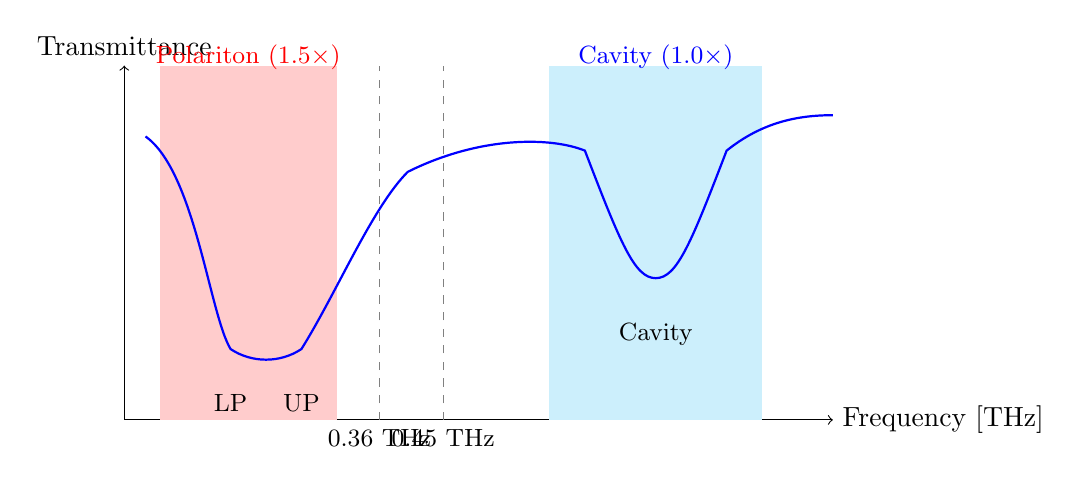
\begin{tikzpicture}[scale=0.9]
    % スペクトル模式図
    \draw[->] (0,0) -- (10,0) node[right] {Frequency [THz]};
    \draw[->] (0,0) -- (0,5) node[above] {Transmittance};
    
    % ポラリトン領域
    \fill[red!20] (0.5,0) rectangle (3,5);
    \node[above, red] at (1.75,4.8) {\small Polariton (1.5$\times$)};
    
    % 共振器領域
    \fill[cyan!20] (6,0) rectangle (9,5);
    \node[above, blue] at (7.5,4.8) {\small Cavity (1.0$\times$)};
    
    % スペクトル曲線
    \draw[thick, blue] (0.3,4) 
        .. controls (1,3.5) and (1.2,1.5) .. (1.5,1)
        .. controls (1.8,0.8) and (2.2,0.8) .. (2.5,1)
        .. controls (3,1.8) and (3.5,3) .. (4,3.5)
        .. controls (5,4) and (6,4) .. (6.5,3.8)
        .. controls (7,2.5) and (7.2,2) .. (7.5,2)
        .. controls (7.8,2) and (8,2.5) .. (8.5,3.8)
        .. controls (9,4.2) and (9.5,4.3) .. (10,4.3);
    
    % ピーク位置のマーカー
    \node[below] at (1.5,0.5) {\small LP};
    \node[below] at (2.5,0.5) {\small UP};
    \node[below] at (7.5,1.5) {\small Cavity};
    
    % 境界線
    \draw[dashed, gray] (3.6,0) -- (3.6,5);
    \node[below] at (3.6,0) {\small 0.36 THz};
    \draw[dashed, gray] (4.5,0) -- (4.5,5);
    \node[below] at (4.5,0) {\small 0.45 THz};
\end{tikzpicture}
\caption{透過スペクトルの領域分類と重み付け。低周波のポラリトン領域には1.5倍の重みを適用。}
\label{fig:weighting}
\end{figure}

%%%%%%%%%%%%%%%%%%%%%%%%%%%%%%%%%%%%%%%%%%%%%%%%%%%%%%%%%%%%%%%%%
\section{プログラムの全体フロー}
%%%%%%%%%%%%%%%%%%%%%%%%%%%%%%%%%%%%%%%%%%%%%%%%%%%%%%%%%%%%%%%%%

\begin{figure}[h]
\centering
\begin{tikzpicture}[
    node distance=1.2cm,
    startstop/.style={rectangle, rounded corners, minimum width=3cm, minimum height=0.8cm, text centered, draw=black, fill=red!30},
    process/.style={rectangle, minimum width=3cm, minimum height=0.8cm, text centered, draw=black, fill=orange!30},
    io/.style={trapezium, trapezium left angle=70, trapezium right angle=110, minimum width=3cm, minimum height=0.8cm, text centered, draw=black, fill=blue!30},
    decision/.style={diamond, minimum width=2cm, minimum height=0.8cm, text centered, draw=black, fill=green!30},
    arrow/.style={thick,->,>=stealth}
]

% ノード
\node (start) [startstop] {開始};
\node (load) [io, below of=start] {データロード (10セット)};
\node (detect) [process, below of=load] {ポラリトン検出・重み付け};
\node (init) [process, below of=detect] {初期値・境界値設定};
\node (opt1) [process, below of=init] {Stage 1: 粗探索};
\node (opt2) [process, below of=opt1] {Stage 2: 中間精緻化};
\node (opt3) [process, below of=opt2] {Stage 3: 微調整};
\node (analyze) [process, below of=opt3] {結果解析・診断};
\node (plot) [io, below of=analyze] {プロット生成・保存};
\node (end) [startstop, below of=plot] {終了};

% 矢印
\draw [arrow] (start) -- (load);
\draw [arrow] (load) -- (detect);
\draw [arrow] (detect) -- (init);
\draw [arrow] (init) -- (opt1);
\draw [arrow] (opt1) -- (opt2);
\draw [arrow] (opt2) -- (opt3);
\draw [arrow] (opt3) -- (analyze);
\draw [arrow] (analyze) -- (plot);
\draw [arrow] (plot) -- (end);

% モデル形式のループ
\node[draw, dashed, fit=(opt1)(opt2)(opt3)(analyze), inner sep=0.3cm, label=right:{\small H形式・B形式で繰り返し}] {};

\end{tikzpicture}
\caption{プログラムの処理フロー}
\label{fig:flowchart}
\end{figure}

%%%%%%%%%%%%%%%%%%%%%%%%%%%%%%%%%%%%%%%%%%%%%%%%%%%%%%%%%%%%%%%%%
\section{出力と診断}
%%%%%%%%%%%%%%%%%%%%%%%%%%%%%%%%%%%%%%%%%%%%%%%%%%%%%%%%%%%%%%%%%

\subsection{フィット品質の評価指標}

\begin{table}[h]
\centering
\caption{評価指標}
\begin{tabular}{lcc}
\toprule
\textbf{指標} & \textbf{定義} & \textbf{良好な基準} \\
\midrule
RMSE & $\sqrt{\frac{1}{N}\sum_i (T_i^{\text{exp}} - T_i^{\text{fit}})^2}$ & $< 0.05$ \\
$R^2$ & $1 - \frac{\sum(T^{\text{exp}} - T^{\text{fit}})^2}{\sum(T^{\text{exp}} - \bar{T})^2}$ & $> 0.95$ \\
Max Error & $\max_i |T_i^{\text{exp}} - T_i^{\text{fit}}|$ & $< 0.15$ \\
$|\chi|_{\max}$ & 感受率の最大絶対値 & $< 0.9$ (B形式) \\
\bottomrule
\end{tabular}
\end{table}

\subsection{物理的診断項目}

\begin{enumerate}
    \item \textbf{基底状態占有率} $p_0$
    \begin{itemize}
        \item $p_0 > 0.95$: 低温で基底状態支配的
        \item 遷移が限られ、フィット自由度が低下
    \end{itemize}
    
    \item \textbf{エネルギーギャップ vs $k_{\text{B}}T$}
    \begin{itemize}
        \item $\Delta E \gg k_{\text{B}}T$: 熱励起が抑制
        \item $\Delta E \ll k_{\text{B}}T$: 多準位が関与
    \end{itemize}
    
    \item \textbf{B形式不安定点}
    \begin{itemize}
        \item $|1-\chi| < 10^{-3}$となる周波数点の割合
        \item $> 5\%$で警告
    \end{itemize}
\end{enumerate}

\subsection{生成される出力ファイル}

\begin{itemize}
    \item \texttt{fit\_all\_spectra.png}: 全スペクトルのフィット結果
    \item \texttt{residuals\_all\_spectra.png}: 残差プロット
    \item \texttt{chi\_distribution.png}: $|\chi|$の周波数分布
    \item \texttt{fit\_statistics.csv}: 統計量一覧
    \item \texttt{diagnostic\_analysis.csv}: 物理診断結果
    \item \texttt{shared\_gamma\_params.json}: 最適パラメータ
\end{itemize}

%%%%%%%%%%%%%%%%%%%%%%%%%%%%%%%%%%%%%%%%%%%%%%%%%%%%%%%%%%%%%%%%%
\section{H形式 vs B形式:どちらを使うべきか}
%%%%%%%%%%%%%%%%%%%%%%%%%%%%%%%%%%%%%%%%%%%%%%%%%%%%%%%%%%%%%%%%%

\begin{table}[h]
\centering
\caption{H形式とB形式の比較}
\begin{tabular}{lcc}
\toprule
\textbf{特性} & \textbf{H形式 $\mu_r = 1 + \chi$} & \textbf{B形式 $\mu_r = 1/(1-\chi)$} \\
\midrule
数値安定性 & 高い(常に安定) & 低い($\chi \to 1$で発散) \\
物理的根拠 & 弱磁化の線形近似 & 強磁化・非線形効果を含む \\
適用条件 & $|\chi| \ll 1$ & $|\chi| \lesssim 1$ でも対応可能 \\
典型的RMSE & やや高い傾向 & やや低い傾向 \\
推奨条件 & 高温・低磁場 & 低温・高磁場 \\
\bottomrule
\end{tabular}
\end{table}

\begin{keypoint}
本プログラムは両形式で計算し、比較プロットを生成します。
物理的状況に応じて適切なモデルを選択してください。
\end{keypoint}

%%%%%%%%%%%%%%%%%%%%%%%%%%%%%%%%%%%%%%%%%%%%%%%%%%%%%%%%%%%%%%%%%
\section{付録:主要関数の説明}
%%%%%%%%%%%%%%%%%%%%%%%%%%%%%%%%%%%%%%%%%%%%%%%%%%%%%%%%%%%%%%%%%

\subsection{get\_hamiltonian}
\begin{lstlisting}[language=Python]
def get_hamiltonian(B_ext_z, g_factor, B4, B6, s=3.5):
    """
    ハミルトニアン行列を構築
    
    Parameters:
        B_ext_z: 外部磁場 [T]
        g_factor: ランデg因子
        B4, B6: 結晶場パラメータ [K]
        s: スピン量子数 (default: 3.5)
    
    Returns:
        H: 8x8 ハミルトニアン行列 [K単位]
    """
\end{lstlisting}

\subsection{calculate\_susceptibility}
\begin{lstlisting}[language=Python]
def calculate_susceptibility(freq_thz, H, T, gamma_thz):
    """
    磁気感受率を計算(全56遷移考慮)
    
    Parameters:
        freq_thz: 周波数配列 [THz]
        H: ハミルトニアン [K]
        T: 温度 [K]
        gamma_thz: 緩和率(7個の配列)[THz]
    
    Returns:
        chi: 複素感受率 (N_freq,)
    """
\end{lstlisting}

\subsection{shared\_gamma\_residuals}
\begin{lstlisting}[language=Python]
def shared_gamma_residuals(params_flat, datasets, model_form='H'):
    """
    全データセットの重み付き残差を計算
    
    Parameters:
        params_flat: スケール済みパラメータ [12個]
        datasets: データセットのリスト
        model_form: 'H' or 'B'
    
    Returns:
        residuals: 全周波数点の残差を連結
    """
\end{lstlisting}

%%%%%%%%%%%%%%%%%%%%%%%%%%%%%%%%%%%%%%%%%%%%%%%%%%%%%%%%%%%%%%%%%
\section{まとめ}
%%%%%%%%%%%%%%%%%%%%%%%%%%%%%%%%%%%%%%%%%%%%%%%%%%%%%%%%%%%%%%%%%

\begin{enumerate}
    \item \textbf{目的}: 複数の実験条件(温度・磁場)で測定した透過スペクトルを、
          物理的に意味のある少数のパラメータで統一的にフィッティング
    
    \item \textbf{核心アイデア}: 7つの緩和率$\gamma_k$を全データセットで共有
          (材料固有の特性として仮定)
    
    \item \textbf{成果}: パラメータ数を75個→12個に削減(84\%減)、
          条件数を$10^{16} \to 10^{6}$に改善
    
    \item \textbf{出力}: H形式・B形式両方での最適パラメータ、
          フィット品質統計、物理診断レポート
\end{enumerate}

\begin{keypoint}
このプログラムは、ベイズ推定(MCMC)の前処理として使用されます。
得られたパラメータは、確率的推定の初期値や事前分布の設計に活用されます。
\end{keypoint}

\end{document}